\documentclass{article}
\usepackage{tikz}
\usetikzlibrary{tikzmark}

%Complex block
\input{cube.tex}
\newcommand{\blockFig}[1]{
  \begin{tikzpicture}
    \tikzcuboid{%
      scale=0.08,%
      densityx=1,%
      densityy=1,%
      densityz=1,%
      dimx=4,%
      dimy=4,%
      dimy=4,%
      linefront=#1!75!black,%
      linetop=#1!50!black,%
      lineright=#1!25!black,%
      fillfront=#1!25!white,%
      filltop=#1!50!white,%
      fillright=#1!75!white,
      emphedge=Y,%
      emphstyle=ultra thin,
    }
  \end{tikzpicture}
}

% Simple block
\newcommand{\simpleBlock}[1]{
  \resizebox{#1pt}{#1pt}{
  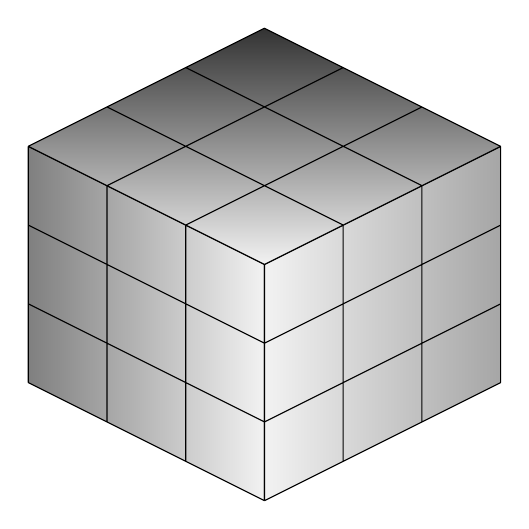
\begin{tikzpicture}
    \shade[yslant=-0.5,right color=gray!10, left color=black!50]
    (0,0) rectangle +(3,3);
    \draw[yslant=-0.5] (0,0) grid (3,3);
    \shade[yslant=0.5,right color=gray!70,left color=gray!10]
    (3,-3) rectangle +(3,3);
    \draw[yslant=0.5] (3,-3) grid (6,0);
    \shade[yslant=0.5,xslant=-1,bottom color=gray!10,
      top color=black!80] (6,3) rectangle +(-3,-3);
    \draw[yslant=0.5,xslant=-1] (3,0) grid (6,3);
  \end{tikzpicture}
  }
}

%Thread
\newcommand{\threadFig}[1]{
  \begin{tikzpicture}
    \vspace{5pt}
    \draw[very thick,color=#1] plot [smooth,tension=1.5] coordinates{(0.3,0.5) (0.25,0.37) (0.3,0.25) (0.25,0.12)};
  \end{tikzpicture}
}

\begin{document}
\begin{figure}
  \center
    \begin{tabular}{ p{15pt} | p{15pt} | p{15pt} | p{15pt} |}
      \cline{2-4}
      \scalebox{0.8}{\blockFig{blue}}  & 1 & 2 & 3\\
      \cline{2-4}
      \scalebox{0.8}{\simpleBlock{15}} & 4 & 5 & 6\\
      \cline{2-4}
    \end{tabular}
\qquad
    \begin{tabular}{ | p{15pt} | p{15pt} | p{15pt} |}
      \multicolumn{1}{c}{\threadFig{blue}} & \multicolumn{1}{c}{\threadFig{blue}} & \multicolumn{1}{c}{\threadFig{blue}}  \\
      \hline
      1 & 2 & 3\\
      \hline
      \multicolumn{1}{c}{\tikzmark{E}} &  \multicolumn{1}{c}{\tikzmark{F}} &  \multicolumn{1}{c}{\tikzmark{G}} \\
    \end{tabular}
\end{figure}

\end{document}
